\documentclass[aspectratio=169]{beamer}

\mode<presentation>
{
  \usetheme{default}
  \usecolortheme{default}
  \usefonttheme{default}
  \setbeamertemplate{navigation symbols}{}
  \setbeamertemplate{caption}[numbered]
  \setbeamertemplate{footline}[frame number]  % or "page number"
  \setbeamercolor{frametitle}{fg=white}
  \setbeamercolor{footline}{fg=black}
} 

\usepackage[english]{babel}
\usepackage[utf8x]{inputenc}
\usepackage{tikz}
\usepackage{courier}
\usepackage{array}
\usepackage{bold-extra}
\usepackage{minted}
\usepackage[thicklines]{cancel}

\xdefinecolor{dianablue}{rgb}{0.18,0.24,0.31}
\xdefinecolor{darkblue}{rgb}{0.1,0.1,0.7}
\xdefinecolor{darkgreen}{rgb}{0,0.5,0}
\xdefinecolor{darkgrey}{rgb}{0.35,0.35,0.35}
\xdefinecolor{darkorange}{rgb}{0.8,0.5,0}
\xdefinecolor{darkred}{rgb}{0.7,0,0}
\definecolor{darkgreen}{rgb}{0,0.6,0}
\definecolor{mauve}{rgb}{0.58,0,0.82}

\title[2018-08-02-maynooth-big-data-software]{Big Data Software in High Energy Physics}
\author{Jim Pivarski}
\institute{Princeton University -- DIANA-HEP}
\date{August 2, 2018}

\begin{document}

\logo{\pgfputat{\pgfxy(0.11, 7.4)}{\pgfbox[right,base]{\tikz{\filldraw[fill=dianablue, draw=none] (0 cm, 0 cm) rectangle (50 cm, 1 cm);}\mbox{\hspace{-8 cm}
\includegraphics[height=1 cm]{princeton-logo-long.png}
\includegraphics[height=1 cm]{diana-hep-logo-long.png}}}}}

\begin{frame}
  \titlepage
\end{frame}

\logo{\pgfputat{\pgfxy(0.11, 7.4)}{\pgfbox[right,base]{\tikz{\filldraw[fill=dianablue, draw=none] (0 cm, 0 cm) rectangle (50 cm, 1 cm);}\mbox{\hspace{-8 cm}
\includegraphics[height=1 cm]{princeton-logo.png}
\includegraphics[height=1 cm]{diana-hep-logo.png}}}}}

% Uncomment these lines for an automatically generated outline.
%\begin{frame}{Outline}
%  \tableofcontents
%\end{frame}

% START START START START START START START START START START START START START

\begin{frame}{What software should you use in your analysis?}
\large
\vspace{0.75 cm}
\begin{columns}
\column{0.53\linewidth}
Sometimes viewed as a vacuous question, like ``What color is your hammer?''

\vspace{0.75 cm}
\uncover<2->{Anything that gets the job done!}
\column{0.4\linewidth}
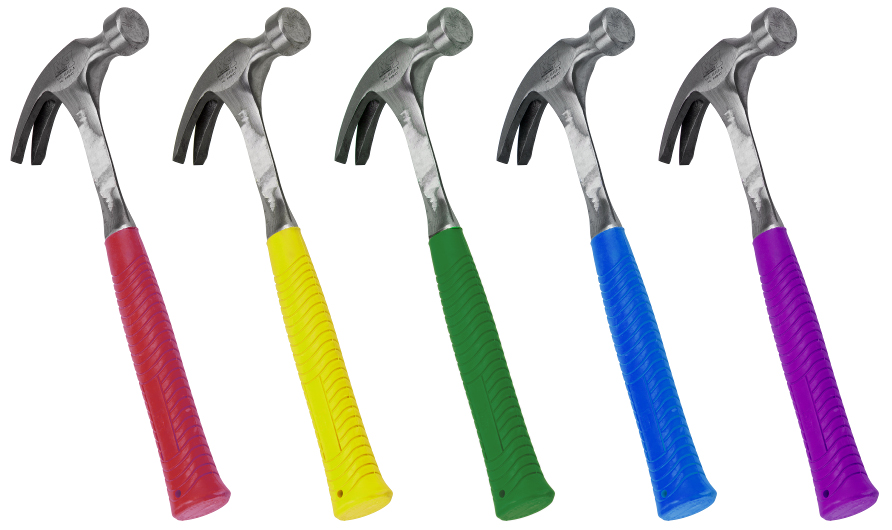
\includegraphics[width=\linewidth]{hammer.jpg}
\end{columns}

\vspace{0.75 cm}
\uncover<3->{\textcolor{darkblue}{But there are real differences and sometimes it matters:}}

\vspace{0.1 cm}
\begin{itemize}\setlength{\itemsep}{0.2 cm}
\item<4-> Tool for the wrong problem \hfill (hammer vs.\ screwdriver)
\item<5-> Ease of use/productivity \hfill (ergonomics of handle)
\item<6-> Computational performance \hfill (sledge hammer weight)
\end{itemize}
\end{frame}

\begin{frame}{}
\vspace{1 cm}
\begin{center}
\Large \textcolor{darkblue}{Why this matters now:}

\vspace{0.5 cm}
\large we're not the only ones analyzing big datasets anymore: ``web scale analytics''
\end{center}
\end{frame}

\begin{frame}{\only<1>{We measure globally distributed data in hundreds of PB}\only<2>{But for ``web scale'' companies, 100 PB = 1 truck}}
\vspace{0.35 cm}
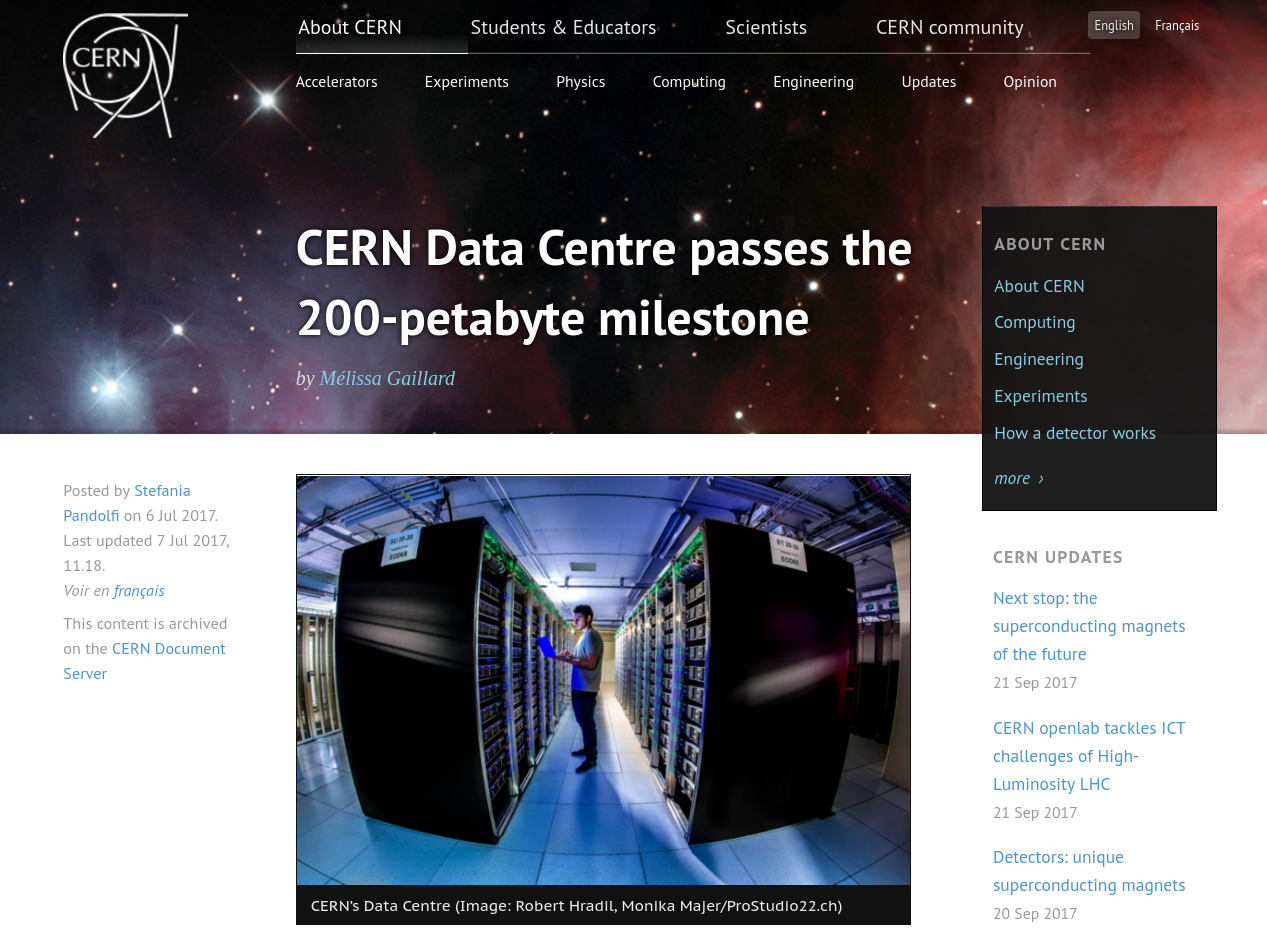
\includegraphics[width=0.73\linewidth]{cern-200pb.png}

\vspace{-4.8 cm}
\uncover<2->{\mbox{ } \hfill 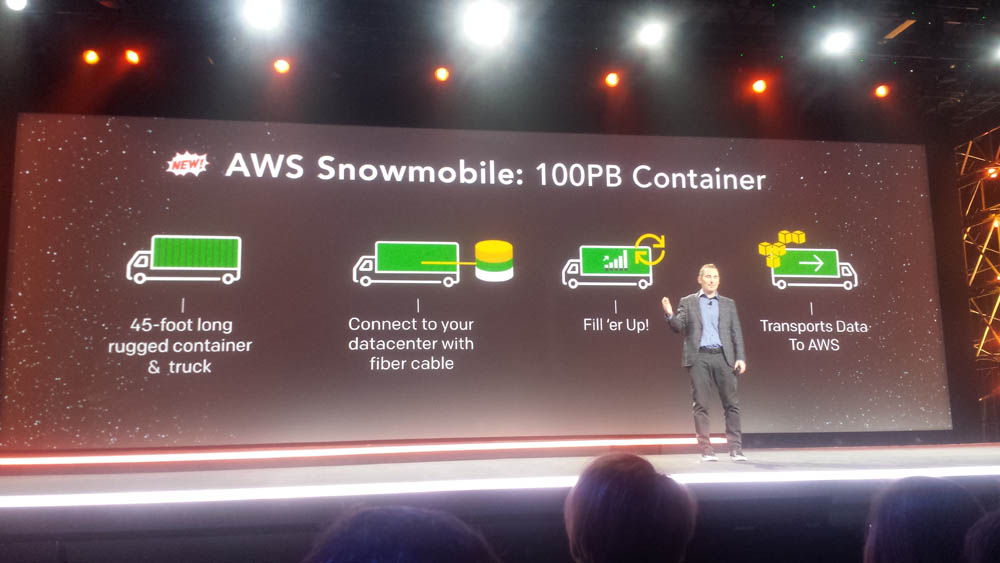
\includegraphics[width=0.7\linewidth]{aws-snowmobile.jpg}\hspace{-1 cm}}
\end{frame}

\begin{frame}{}
\vspace{1 cm}
\large
\begin{columns}[t]
\column{0.5\linewidth}
\textcolor{darkblue}{\underline{What we can find off the shelf}}

\vspace{0.1 cm}
\begin{itemize}\setlength{\itemsep}{0.1 cm}
\item distributed processing, scale-out
\item C++/Python interoperability
\item special functions, matrix math
\item fitting/minimization, integration, differentiation, interpolation
\item symbolic algebra
\item advanced statistics
\item machine learning
\item graphics, advanced plotting
\item graphical interfaces, user workflows
\end{itemize}

\column{0.5\linewidth}
\textcolor{darkblue}{\underline{What we still must develop in-house}}

\vspace{0.1 cm}
\begin{itemize}\setlength{\itemsep}{0.1 cm}
\item reading/writing ROOT files
\item collaboration frameworks, event reconstruction
\item advanced histogramming and fitting
\item efficient variable-length lists (our kind of non-relational data)
\item domain-specific functions
\end{itemize}
\end{columns}
\end{frame}





\end{document}
